\documentclass[11pt,a4paper]{article}

\usepackage[utf8]{inputenc}
\usepackage[T1]{fontenc}
\usepackage[romanian]{babel}
\usepackage{lmodern}
\usepackage[margin=2.3cm]{geometry}
\usepackage{tabularx}
\usepackage{booktabs}
\usepackage{array}
\usepackage{enumitem}
\usepackage{xcolor}
\usepackage{tikz}
\usetikzlibrary{positioning,arrows.meta,fit,backgrounds}
\usepackage[hidelinks]{hyperref}
\usepackage{parskip}

\definecolor{accent}{HTML}{2F6FDB}
\definecolor{accentbg}{HTML}{E6EEFB}
\definecolor{bordercol}{HTML}{B8B8B0}
\definecolor{tintbg}{HTML}{EEEEEB}
\definecolor{quiet}{HTML}{5F5F5A}

\renewcommand{\arraystretch}{1.3}
\newcolumntype{L}{>{\raggedright\arraybackslash}X}
\setlist{itemsep=2pt, topsep=4pt}

\title{\textbf{Prezentare generală -- Platformă de accesibilitate pentru persoane surde}}
\author{}
\date{22 octombrie 2026}

\begin{document}
\maketitle
\vspace{-1.5em}

% ------------------------------------------------------------
\section*{Rezumat}

Construim o platformă care face meetingurile față în față accesibile persoanelor surde și cu deficiențe de auz: vezi cine vorbește, citești tot ce se spune și poți interveni fără să întrerupi. Același motor (microfon, cameră, AI rulat local) alimentează două funcții bonus: subtitrări pentru conversațiile de zi cu zi și alerte vizuale pentru sunetele de siguranță de la locul de muncă.

\begin{center}
\begin{tabularx}{\textwidth}{>{\raggedright\arraybackslash}p{4.2cm} >{\raggedright\arraybackslash}p{3cm} L}
\toprule
\textbf{Componentă} & \textbf{Rol} & \textbf{Problema rezolvată} \\
\midrule
Asistentul pentru meetinguri & Soluția principală & Persoana surdă pierde ce se spune și nu poate interveni ușor într-un meeting fizic \\
Subtitrări în lumea reală & Funcție bonus 1 & Conversațiile informale (cafea, brief de tură, birou) rămân fără subtitrare \\
Sunetul vizibil & Funcție bonus 2 & Alarmele, claxoanele și strigătele nu sunt auzite, deci postul fizic devine riscant \\
\bottomrule
\end{tabularx}
\end{center}

\textbf{Pentru cine:} angajați și studenți surzi sau cu deficiențe de auz, angajatorii lor (HR, responsabili de siguranță) și organizatorii de meetinguri, cursuri și evenimente.

% ------------------------------------------------------------
\section*{Problema și contextul pieței}

Subtitrarea live există, dar e construită în jurul unui singur telefon ținut aproape de vorbitor sau în jurul apelurilor online. Meetingul fizic, cu un prezentator în față și public în sală, rămâne slab acoperit.

Ce există azi:
\begin{itemize}
  \item \href{https://ava.me/blog/ava-vs-ai-media-the-ultimate-solution-for-live-captioning-needs}{Ava} colorează și etichetează vorbitorii și oferă Ava Voice (text tastat citit cu voce tare). Pentru grupuri față în față recomandă ca ceilalți să instaleze aplicația, iar telefonul trebuie ținut la 30--60 cm de vorbitor (\href{https://help.ava.me/en/articles/3157495-use-ava-to-caption-someone-face-to-face}{ghid Ava}).
  \item \href{https://apps.appfollow.io/ios/live-transcribe/1471473738?country=it}{Live Transcribe (Mighty Fine Apps)} are detectare de vorbitori cu cuvinte colorate.
  \item \href{https://www.hearingtracker.com/hearing-glasses/hear-with-your-eyes-five-ar-live-captioning-glasses}{XRAI} afișează subtitrări pe telefon sau ochelari AR, cu identificare de vorbitor în planul plătit. Utilizatorii raportează că merge bine doar când vorbește câte unul (\href{https://forum.hearingtracker.com/t/captioning-glasses-e-g-xrai-state-of-market-as-of-jan-26/110090}{forum HearingTracker}).
  \item \href{https://apps.apple.com/app/id6450253525}{Conference Live Captioning} transmite subtitrarea vorbitorului către telefoanele participanților, fără canal înapoi.
\end{itemize}

Ce lipsește: un al doilea dispozitiv pus lângă prezentator, notificarea silențioasă către acesta, identificarea rolurilor (prezentator vs.\ public) cu ajutorul camerei și opțiuni combinate pentru dislexie și daltonism. Recomandările pentru meetinguri accesibile cer explicit ca participanții să ridice mâna, ca persoana surdă să vadă cine urmează să vorbească (\href{https://rnid.org.uk/employers-and-professionals/accessible-meetings/}{RNID}); produsul nostru face asta automat.

% ------------------------------------------------------------
\section*{Soluția principală: Asistentul pentru meetinguri}

Persoana surdă urmărește tot meetingul ca pe un film subtitrat, știe mereu cine vorbește și poate trimite o întrebare direct prezentatorului, fără să întrerupă.

\subsection*{1. Scanarea sălii}
La pornire, camera scanează sala și detectează fețele și pozițiile. Aplicația marchează automat coordonatorul (persoana de la pupitru sau din fața sălii), iar utilizatorul poate corecta cu un tap. De aici încolo, fiecare replică e atribuită fie coordonatorului, fie unei persoane din public.

\subsection*{2. Două moduri de folosire}
\begin{center}
\begin{tabularx}{\textwidth}{>{\raggedright\arraybackslash}p{3cm} L L}
\toprule
\textbf{Mod} & \textbf{Configurare} & \textbf{Când se potrivește} \\
\midrule
Un singur dispozitiv & Telefonul sau laptopul utilizatorului ascultă și filmează sala & Meetinguri mici, sală mică, setup rapid \\
Două dispozitive & Laptopul stă în fața prezentatorului (microfon apropiat + ecran de notificări); telefonul rămâne la utilizator & Prezentări, cursuri, săli mari, unde vocea prezentatorului se pierde de la distanță \\
\bottomrule
\end{tabularx}
\end{center}
În modul cu două dispozitive, cele două se conectează printr-un cod QR sau un cod scurt, fără cont pentru prezentator.

\subsection*{3. Notificare către prezentator}
Utilizatorul tastează o întrebare sau alege un mesaj rapid („Am o întrebare”, „Puteți repeta?”, „Mai rar, vă rog”). Mesajul apare discret pe laptopul prezentatorului, ca notificare, fără sunet. Opțional, poate fi citit cu voce tare când prezentatorul îi dă cuvântul.

\subsection*{4. Subtitrare cu roluri și culori}
\begin{itemize}
  \item Tot ce se spune cu sens e transformat în text în timp real; zgomotele și discuțiile de fundal sunt filtrate.
  \item Coordonatorul are o culoare și o poziție fixă (de exemplu, sus); vocile din public apar în alte culori, cu etichetă (Public 1, Public 2).
  \item La final: transcriere completă, rezumat și lista de sarcini.
\end{itemize}

\subsection*{5. Accesibilitate vizuală}
\begin{itemize}
  \item \textbf{Daltonism:} palete testate pentru protanopie, deuteranopie și tritanopie; rolul nu depinde doar de culoare, ci și de iconiță, poziție și etichetă.
  \item \textbf{Dislexie:} font dedicat (de exemplu OpenDyslexic), spațiere mai mare între rânduri și litere, viteză de derulare reglabilă.
  \item Mărime text, contrast ridicat și temă întunecată.
\end{itemize}

% ------------------------------------------------------------
\section*{Funcție bonus 1: Subtitrări în lumea reală}

Aceeași tehnologie din meeting merge și în afara lui: la cafea, la brief-ul de tură sau când șeful explică ceva la birou, fiecare replică apare ca un balon lângă fața celui care vorbește.

\textbf{Problema:} subtitrările există pentru Zoom și Teams, dar conversațiile față în față, informale, rămân inaccesibile.

\textbf{Cum funcționează:}
\begin{enumerate}
  \item Utilizatorul ține telefonul sau laptopul îndreptat spre interlocutori.
  \item Camera detectează fețele (de exemplu cu MediaPipe, direct în browser) și identifică cine vorbește după mișcarea buzelor.
  \item Subtitrarea apare ca balon de benzi desenate lângă fața vorbitorului, deci e clar cine ce a spus, chiar și când vorbesc mai mulți.
  \item Un al doilea strat afișează o variantă simplificată a textului.
  \item La final, AI-ul extrage sarcinile din conversație.
\end{enumerate}

\textbf{Legătura cu soluția principală:} e modul „un singur dispozitiv” al asistentului, fără prezentator și fără notificări, gândit pentru grupuri mici și conversații spontane.

% ------------------------------------------------------------
\section*{Funcție bonus 2: Sunetul vizibil}

Telefonul devine „urechea” de siguranță a angajatului surd: recunoaște alarmele, claxoanele și strigătele și le transformă în alerte vizuale și vibrații, în funcție de urgență.

\textbf{Problema:} într-un depozit, magazin sau fabrică, un angajat surd nu aude alarma de incendiu, claxonul stivuitorului, telefonul sau colegul care îl strigă. E o problemă de siguranță și unul dintre motivele pentru care angajatorii evită să angajeze persoane surde pe posturi fizice.

\textbf{Cum funcționează:}
\begin{itemize}
  \item Telefonul sau laptopul ascultă continuu, iar un model de clasificare audio (de exemplu YAMNet, care rulează și în browser) funcționează local, pe dispozitiv.
  \item Recunoaște sunetele relevante: alarmă, sirenă, claxon, numele utilizatorului, telefon, ușă.
  \item Când cineva începe să vorbească cu utilizatorul, pornește automat subtitrarea live.
  \item \textbf{Antrenare pe locație:} HR-ul înregistrează 3--5 mostre din sunetele specifice (alarma lor, semnalul liniei de producție), iar modelul le învață.
\end{itemize}

\textbf{Niveluri de alertă:}
\begin{center}
\begin{tabularx}{\textwidth}{>{\raggedright\arraybackslash}p{2.2cm} >{\raggedright\arraybackslash}p{4.3cm} L}
\toprule
\textbf{Nivel} & \textbf{Exemple} & \textbf{Ce primește utilizatorul} \\
\midrule
Critic & Alarmă de incendiu, sirenă & Ecran complet roșu, vibrație continuă, mesaj „ALARMĂ DE INCENDIU” + ieșirea cea mai apropiată \\
Atenție & Claxon de stivuitor, semnal de linie & Banner colorat, vibrație puternică, pe telefon și ceas \\
Informativ & Numele strigat, telefon, ușă & Notificare discretă, vibrație scurtă \\
\bottomrule
\end{tabularx}
\end{center}

\textbf{Legătura cu soluția principală:} poate rula în fundal și în timpul meetingului, deci o alarmă întrerupe subtitrarea indiferent ce face utilizatorul.

% ------------------------------------------------------------
\section*{Cum se leagă componentele}

Toate cele trei funcții folosesc același motor, care rulează pe telefon sau laptop: o singură aplicație, o singură instalare, un singur model de confidențialitate.

\begin{center}
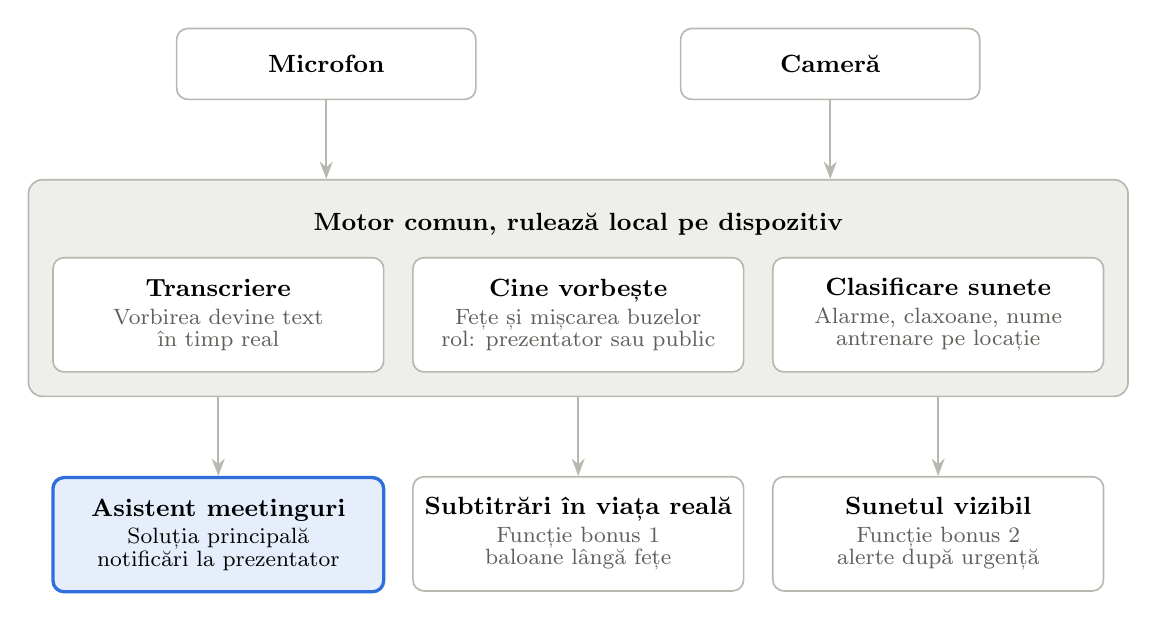
\begin{tikzpicture}[
  font=\small,
  box/.style={draw=bordercol, rounded corners=4pt, line width=0.6pt, align=center,
              minimum width=4.2cm, minimum height=1.45cm, fill=white},
  inbox/.style={draw=bordercol, rounded corners=4pt, line width=0.6pt,
                minimum width=3.8cm, minimum height=0.9cm, font=\small\bfseries, fill=white},
  main/.style={box, draw=accent, fill=accentbg, line width=1.2pt},
  arr/.style={-{Stealth[length=2.2mm]}, draw=bordercol, line width=0.7pt}
]
  % module
  \node[box] (m1) {\textbf{Transcriere}\\[-1pt]{\footnotesize\color{quiet}Vorbirea devine text}\\[-3pt]{\footnotesize\color{quiet}în timp real}};
  \node[box, right=0.35cm of m1] (m2) {\textbf{Cine vorbește}\\[-1pt]{\footnotesize\color{quiet}Fețe și mișcarea buzelor}\\[-3pt]{\footnotesize\color{quiet}rol: prezentator sau public}};
  \node[box, right=0.35cm of m2] (m3) {\textbf{Clasificare sunete}\\[-1pt]{\footnotesize\color{quiet}Alarme, claxoane, nume}\\[-3pt]{\footnotesize\color{quiet}antrenare pe locație}};

  % containerul motorului
  \node[above=0.15cm of m2, font=\small\bfseries] (title) {Motor comun, rulează local pe dispozitiv};
  \begin{scope}[on background layer]
    \node[draw=bordercol, fill=tintbg, rounded corners=5pt, line width=0.6pt,
          inner sep=0.3cm, fit=(m1)(m2)(m3)(title)] (engine) {};
  \end{scope}

  % intrari
  \node[inbox, above=1.0cm of engine.north, xshift=-3.2cm] (mic) {Microfon};
  \node[inbox, above=1.0cm of engine.north, xshift=3.2cm] (cam) {Cameră};
  \draw[arr] (mic.south) -- (mic.south |- engine.north);
  \draw[arr] (cam.south) -- (cam.south |- engine.north);

  % iesiri
  \node[main, below=1.0cm of engine.south -| m1] (o1) {\textbf{Asistent meetinguri}\\[-1pt]{\footnotesize Soluția principală}\\[-3pt]{\footnotesize notificări la prezentator}};
  \node[box, below=1.0cm of engine.south -| m2] (o2) {\textbf{Subtitrări în viața reală}\\[-1pt]{\footnotesize\color{quiet}Funcție bonus 1}\\[-3pt]{\footnotesize\color{quiet}baloane lângă fețe}};
  \node[box, below=1.0cm of engine.south -| m3] (o3) {\textbf{Sunetul vizibil}\\[-1pt]{\footnotesize\color{quiet}Funcție bonus 2}\\[-3pt]{\footnotesize\color{quiet}alerte după urgență}};
  \draw[arr] (o1.north |- engine.south) -- (o1.north);
  \draw[arr] (o2.north |- engine.south) -- (o2.north);
  \draw[arr] (o3.north |- engine.south) -- (o3.north);
\end{tikzpicture}
\end{center}

Asistentul pentru meetinguri folosește transcrierea și identificarea vorbitorului; subtitrările în viața reală adaugă baloanele lângă fețe; sunetul vizibil folosește clasificarea sunetelor și poate rula în fundal în orice mod.

\textbf{Confidențialitate:} audio și video sunt procesate local, nu se trimit pe server. Transcrierile se salvează pe dispozitiv doar dacă utilizatorul alege asta.

% ------------------------------------------------------------
\section*{Diferențiere față de concurență}

Concurenții acoperă subtitrarea și identificarea vorbitorului; noi adăugăm structura meetingului (prezentator vs.\ public), canalul silențios către prezentator și siguranța la locul de muncă.

\begin{center}
\small
\begin{tabularx}{\textwidth}{>{\raggedright\arraybackslash}p{4.3cm} L L L L}
\toprule
\textbf{Funcție} & \textbf{Noi} & \textbf{Ava} & \textbf{XRAI} & \textbf{Live Transcribe} \\
\midrule
Subtitrare live colorată pe vorbitori & Da & Da & Da (plan plătit) & Da \\
Roluri prezentator / public & Da, din cameră & Nu & Nu & Nu \\
Mod cu două dispozitive (laptop la prezentator) & Da & Nu & Parțial (XRAI Stream) & Nu \\
Notificare silențioasă către prezentator & Da & Nu (voce cu glas tare) & Nu & Nu \\
Balon lângă fața vorbitorului & Da & Nu & Nu & Nu \\
Alerte de siguranță antrenate pe locație & Da & Doar zgomote generale & Nu & Nu \\
Mod dislexie + daltonism integrat & Da & Neconfirmat & Neconfirmat & Neconfirmat \\
\bottomrule
\end{tabularx}
\end{center}

{\small\color{quiet} Datele despre concurenți provin din materialele lor publice; „neconfirmat” înseamnă că nu am găsit informația, nu că funcția lipsește sigur.}

% ------------------------------------------------------------
\section*{Demo pentru juriu, scalabilitate și roadmap}

Demo-ul are trei momente scurte, câte unul pentru fiecare componentă, în ordinea importanței.

\textbf{Scenariul demo:}
\begin{enumerate}
  \item \textbf{Meeting:} un coleg prezintă cu laptopul în față, altul pune o întrebare din „public”. Pe telefonul utilizatorului replicile apar în culori diferite, cu rolul marcat. Utilizatorul trimite „Am o întrebare”, iar mesajul apare instant pe laptopul prezentatorului.
  \item \textbf{Conversație:} doi membri ai echipei discută în fața juriului, iar balonul fiecăruia apare lângă fața lui, în timp real.
  \item \textbf{Siguranță:} se pornește o alarmă de incendiu dintr-un difuzor. Telefonul vibrează, ecranul devine roșu cu mesajul „ALARMĂ DE INCENDIU -- ieșirea cea mai apropiată: \ldots”.
\end{enumerate}

\textbf{Scalabilitate:}
\begin{itemize}
  \item Procesarea locală nu costă server și nu trimite audio nicăieri: avantaj de cost și de confidențialitate.
  \item Fiecare locație își antrenează propriile sunete, deci aplicația se adaptează oricărui spațiu de lucru.
  \item Funcționează pe dispozitive pe care oamenii le au deja (telefon, laptop), fără hardware dedicat.
\end{itemize}

\textbf{Roadmap:}
\begin{enumerate}
  \item \textbf{MVP:} asistentul pentru meetinguri cu un dispozitiv și cu două dispozitive, subtitrare colorată, notificare la prezentator, mod dislexie și daltonism.
  \item \textbf{Bonusuri:} baloane lângă fețe pentru conversații și alertele de sunet cu antrenare pe locație.
  \item \textbf{Companii:} panou pentru HR, conturi pe organizație, integrare cu ceasuri inteligente.
  \item \textbf{Viitor:} același motor pe ochelari AR, cu subtitrarea în câmpul vizual.
\end{enumerate}

\end{document}
